\subsection{Cooperatively bound tau uniquely interacts with microtubule motor proteins and cutting enzymes}
\begin{figure}[h!]
\centering
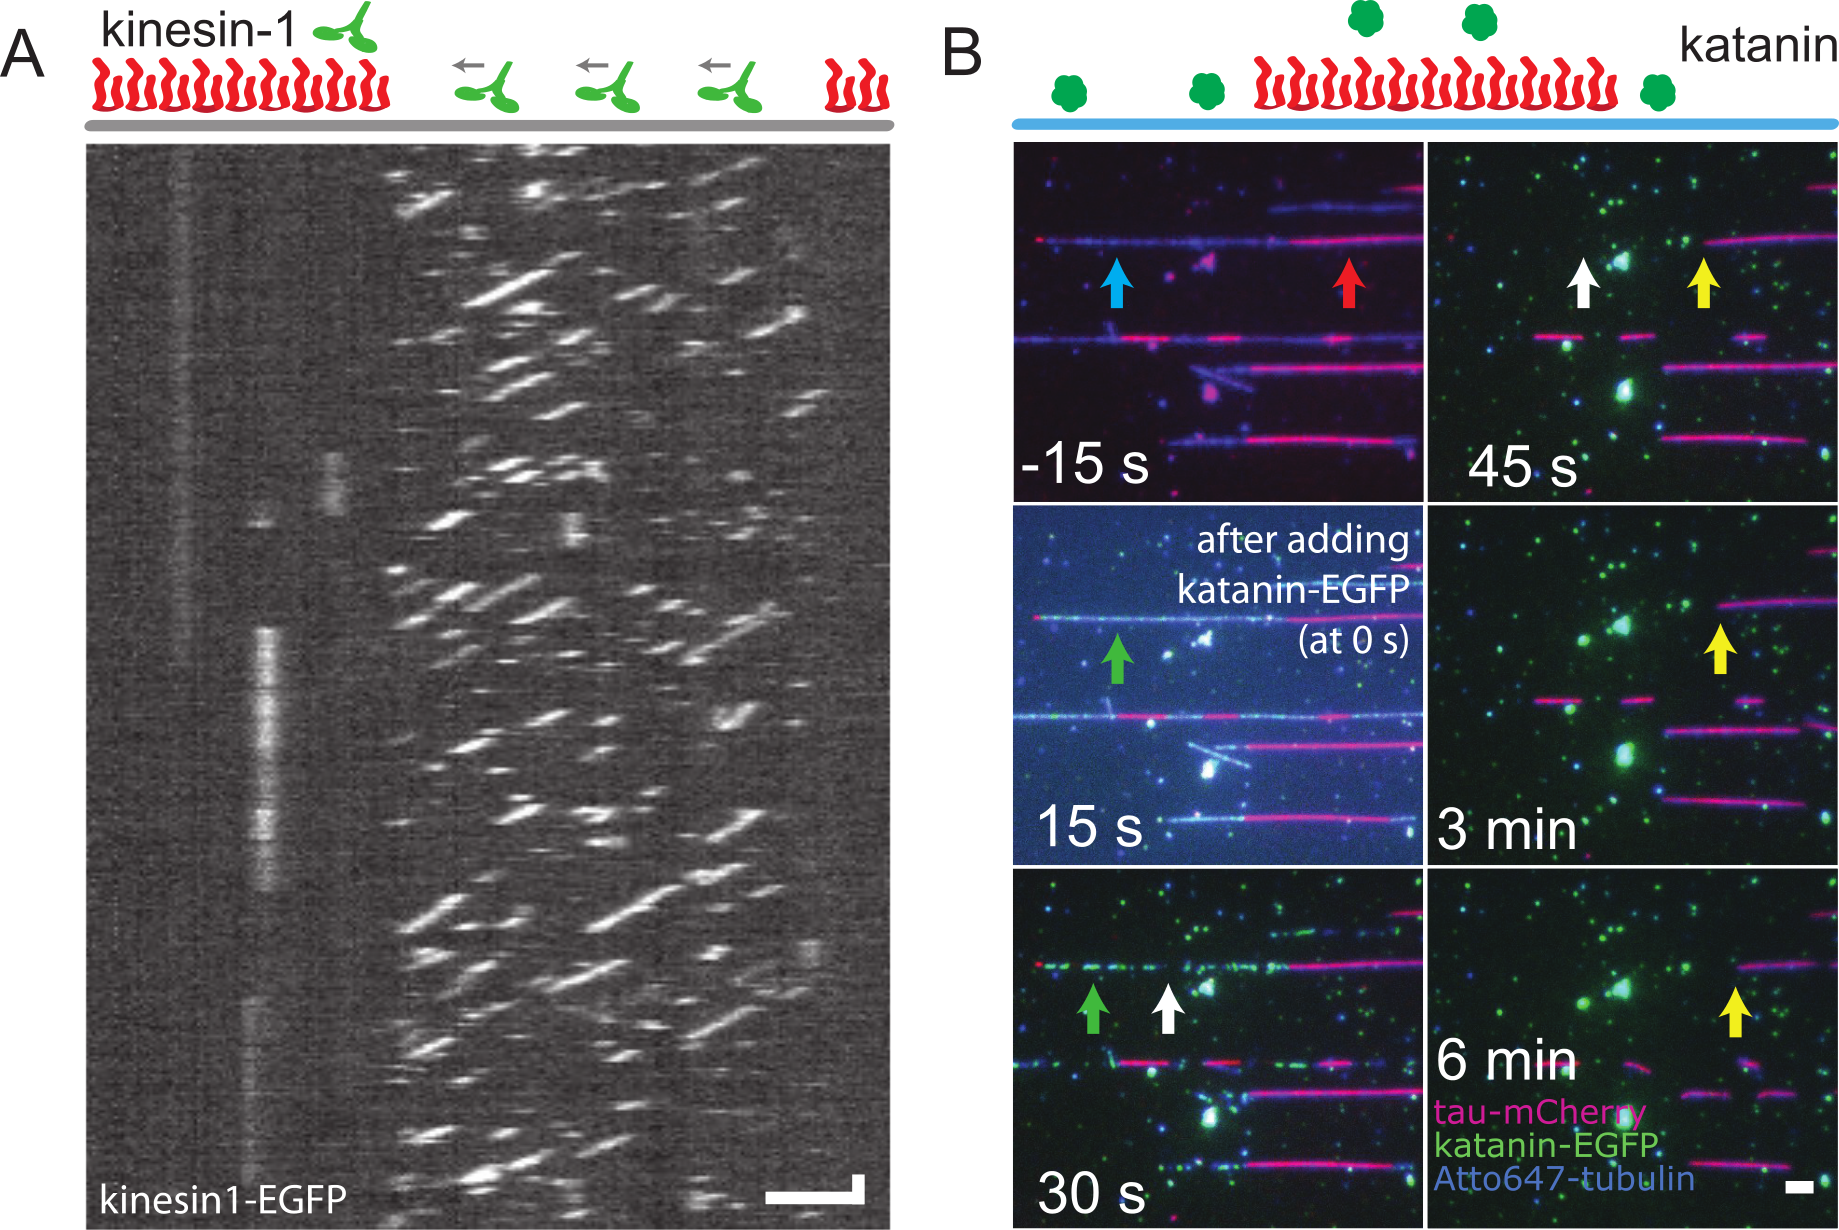
\includegraphics[width=1\linewidth]{Figures/tau3.png}
\caption[Tau islands constitute a protective sheath around microtubules.]{
\textbf{Tau islands constitute a protective sheath around microtubules.} (A) Intensity-inverted kymograph showing kinesin-1-GFP molecules bind to and move processively outside of the islands (the positions of the islands are indicated by schematics above the kymograph). We observed no kinesin-1-GFP binding within the island regions. When reaching the island boundaries, the kinesin-1-GFP molecules immediately dissociate from the microtubule. (B) Fluorescence micrographs showing the katanin-GFP-driven (green, position indicated by green arrow) severing of Atto-647-microtubules (blue) decorated with tau-mCherry islands (red, position indicated by red arrow) interspersed by regions of low tau-mEGFP density (indicated by blue arrow). Initially, microtubule severing and microtubule disassembly occurred only in the regions surrounding the islands (e.g. indicated by white arrow). On longer time scales (after approximately 1 minute), when the microtubule regions not protected by the islands already disassembled, katanin-GFP induced shortening of the island-covered regions of the microtubule (e.g. indicated by yellow arrow). Scale bars, vertical 2 s, horizontal 2 µm.   
	}\label{tau3}
\end{figure}
To investigate how the presence of tau islands affects the interaction of other proteins with microtubules, we formed tau islands using tau-mCherry and tested the interaction of other axonal MAPs with such tau-mCherry-decorated microtubules. First, we tested the processive microtubule-transport motor, kinesin-1. After addition of 60 nM kinesin-1 (GFP-tagged, dimerizing, truncated to be constitutively active, R. norvegicus kinesin-1: rKin-430-GFP) to microtubules in the presence of 20 nM tau-mCherry, we observed single motors moving processively through the low-density tau regions surrounding the islands. However, when reaching the boundary of a tau island, the motors dissociated instantaneously from the microtubule (Figure \ref{tau3}A). No motors bound to the tau islands from solution, resulting in rKin-430-GFP localizing solely to the surroundings of the islands. These results show that tau islands prevent kinesin-1-mediated transport along the microtubule surface. Second, we tested how the presence of islands affects the microtubule-severing enzyme katanin. After the addition of 100 nM katanin (GFP-tagged, M. musculus katanin p60/p80C: katanin-GFP\parencite{Jiang2017} to microtubules in the presence of 20 nM tau-mCherry, we observed katanin-GFP binding, severing and subsequent microtubule disassembly exclusively in the low-density tau regions surrounding the islands (Figure \ref{tau3}B). Only on longer time scales, the island-sheathed regions of the microtubules started to disassemble from their boundaries (Figure \ref{tau3}B), demonstrating that island-generated tau sheaths grant access to the microtubules only at their boundaries. Combined, these results show that tau islands constitute a protective sheath around the microtubule surface, which can hinder the activity of microtubule-severing factors and block kinesin-1-based transport. 

\begin{figure}[h!]
\centering
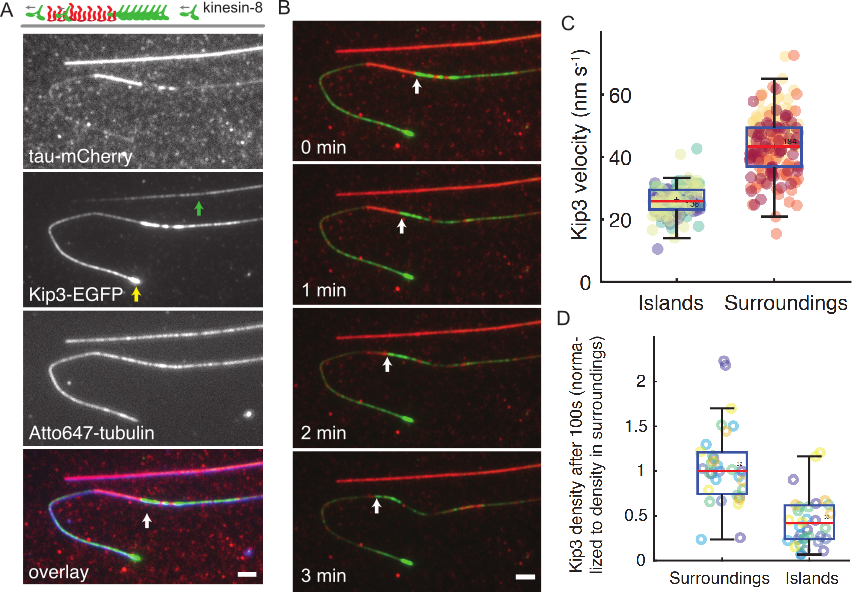
\includegraphics[scale=0.63]{Figures/tau4.png}
\caption[Tau islands can be regulated by super-processive kinesin motors.]{
\textbf{Tau islands can be regulated by super-processive kinesin motors.} (A) Multichannel fluorescence micrographs showing that kip3-GFP (kinesin-8, green) localizes in both regions, outside and within the tau-mCherry (red) islands (indicated by green arrow) on Atto-647-labeled microtubules (blue) and accumulates at the microtubule ends (yellow arrow) and in front of the islands (white arrow). (B) Multicolor timelapse micrographs showing that kip3-GFP (green) accumulating in front of the tau-mCherry island (red), can remove the island by displacing the tau-mCherry from the island edge (receding of the island boundary indicated by white arrow). (C) Quantification of velocities of single Kip3-GFP motors moving inside and outside the islands at 10 nM tau-mCherry in solution (n = 136 Kip3-GFP molecules inside islands, n = 184 outside, 3 experiments). (D) Quantification of Kip3-GFP density inside and outside the islands 100 s after the addition of Kip3-GFP (n = 98 microtubules in 6 experiments). The presented Kip3-GFP densities are normalized to the median of the density in the surroundings (within the same experiment).  Scale bars 2 µm.  
	}\label{tau4}
\end{figure}
To explore the effect of the tau islands on other kinesin family members, we turned to kinesin-8, which is involved in regulating axonal microtubule dynamics\parencite{KEVENAAR2016849}. S. cerevisiae Kip3, the best described member of the kinesin-8 family, pauses for extended periods of time when there is no available binding site within reach\parencite{Varga2009} resulting in its super-processivity\parencite{Varga2006} and the formation of traffic jams at the end of microtubules\parencite{Leduc2012}. Microtubule interaction sites of kinesin motor domains and the microtubule binding repeats of tau partially overlap\parencite{Kellogg2018}. We therefore wondered if (i) traffic jams would form in front of tau islands, where the Kip3 binding sites are occupied by the microtubule binding repeats of tau, and (ii) what effect high-density accumulations of molecular motors might have on tau islands. We thus tested the interaction of 45 nM Kip3-GFP with microtubules decorated with tau islands formed at 10 nM tau-mCherry. After the addition of Kip3-GFP, we observed that Kip3-GFP molecules could move in the low-density tau regions, like kinesin-1, and, in contrast to kinesin-1, also within the tau islands, albeit at a decreased velocity (Figure \ref{tau4}). Importantly, we observed that Kip3-GFP accumulated, in the direction of its movement, at the boundaries of the tau islands. Such high-density traffic jams of accumulated Kip3-GFP caused enhanced unbinding of tau-mCherry at these positions, eventually leading to the complete removal of the islands (Figures \ref{tau4}A,B and \ref{tau_s4}). The island displacement by Kip3 shows that not only do tau islands regulate the interaction of other MAPs with the microtubule surface but that, vice versa, the activity of other MAPs, such as super-processive motors proteins, can regulate the dynamics of the islands themselves.

\begin{figure}[h!]
\centering
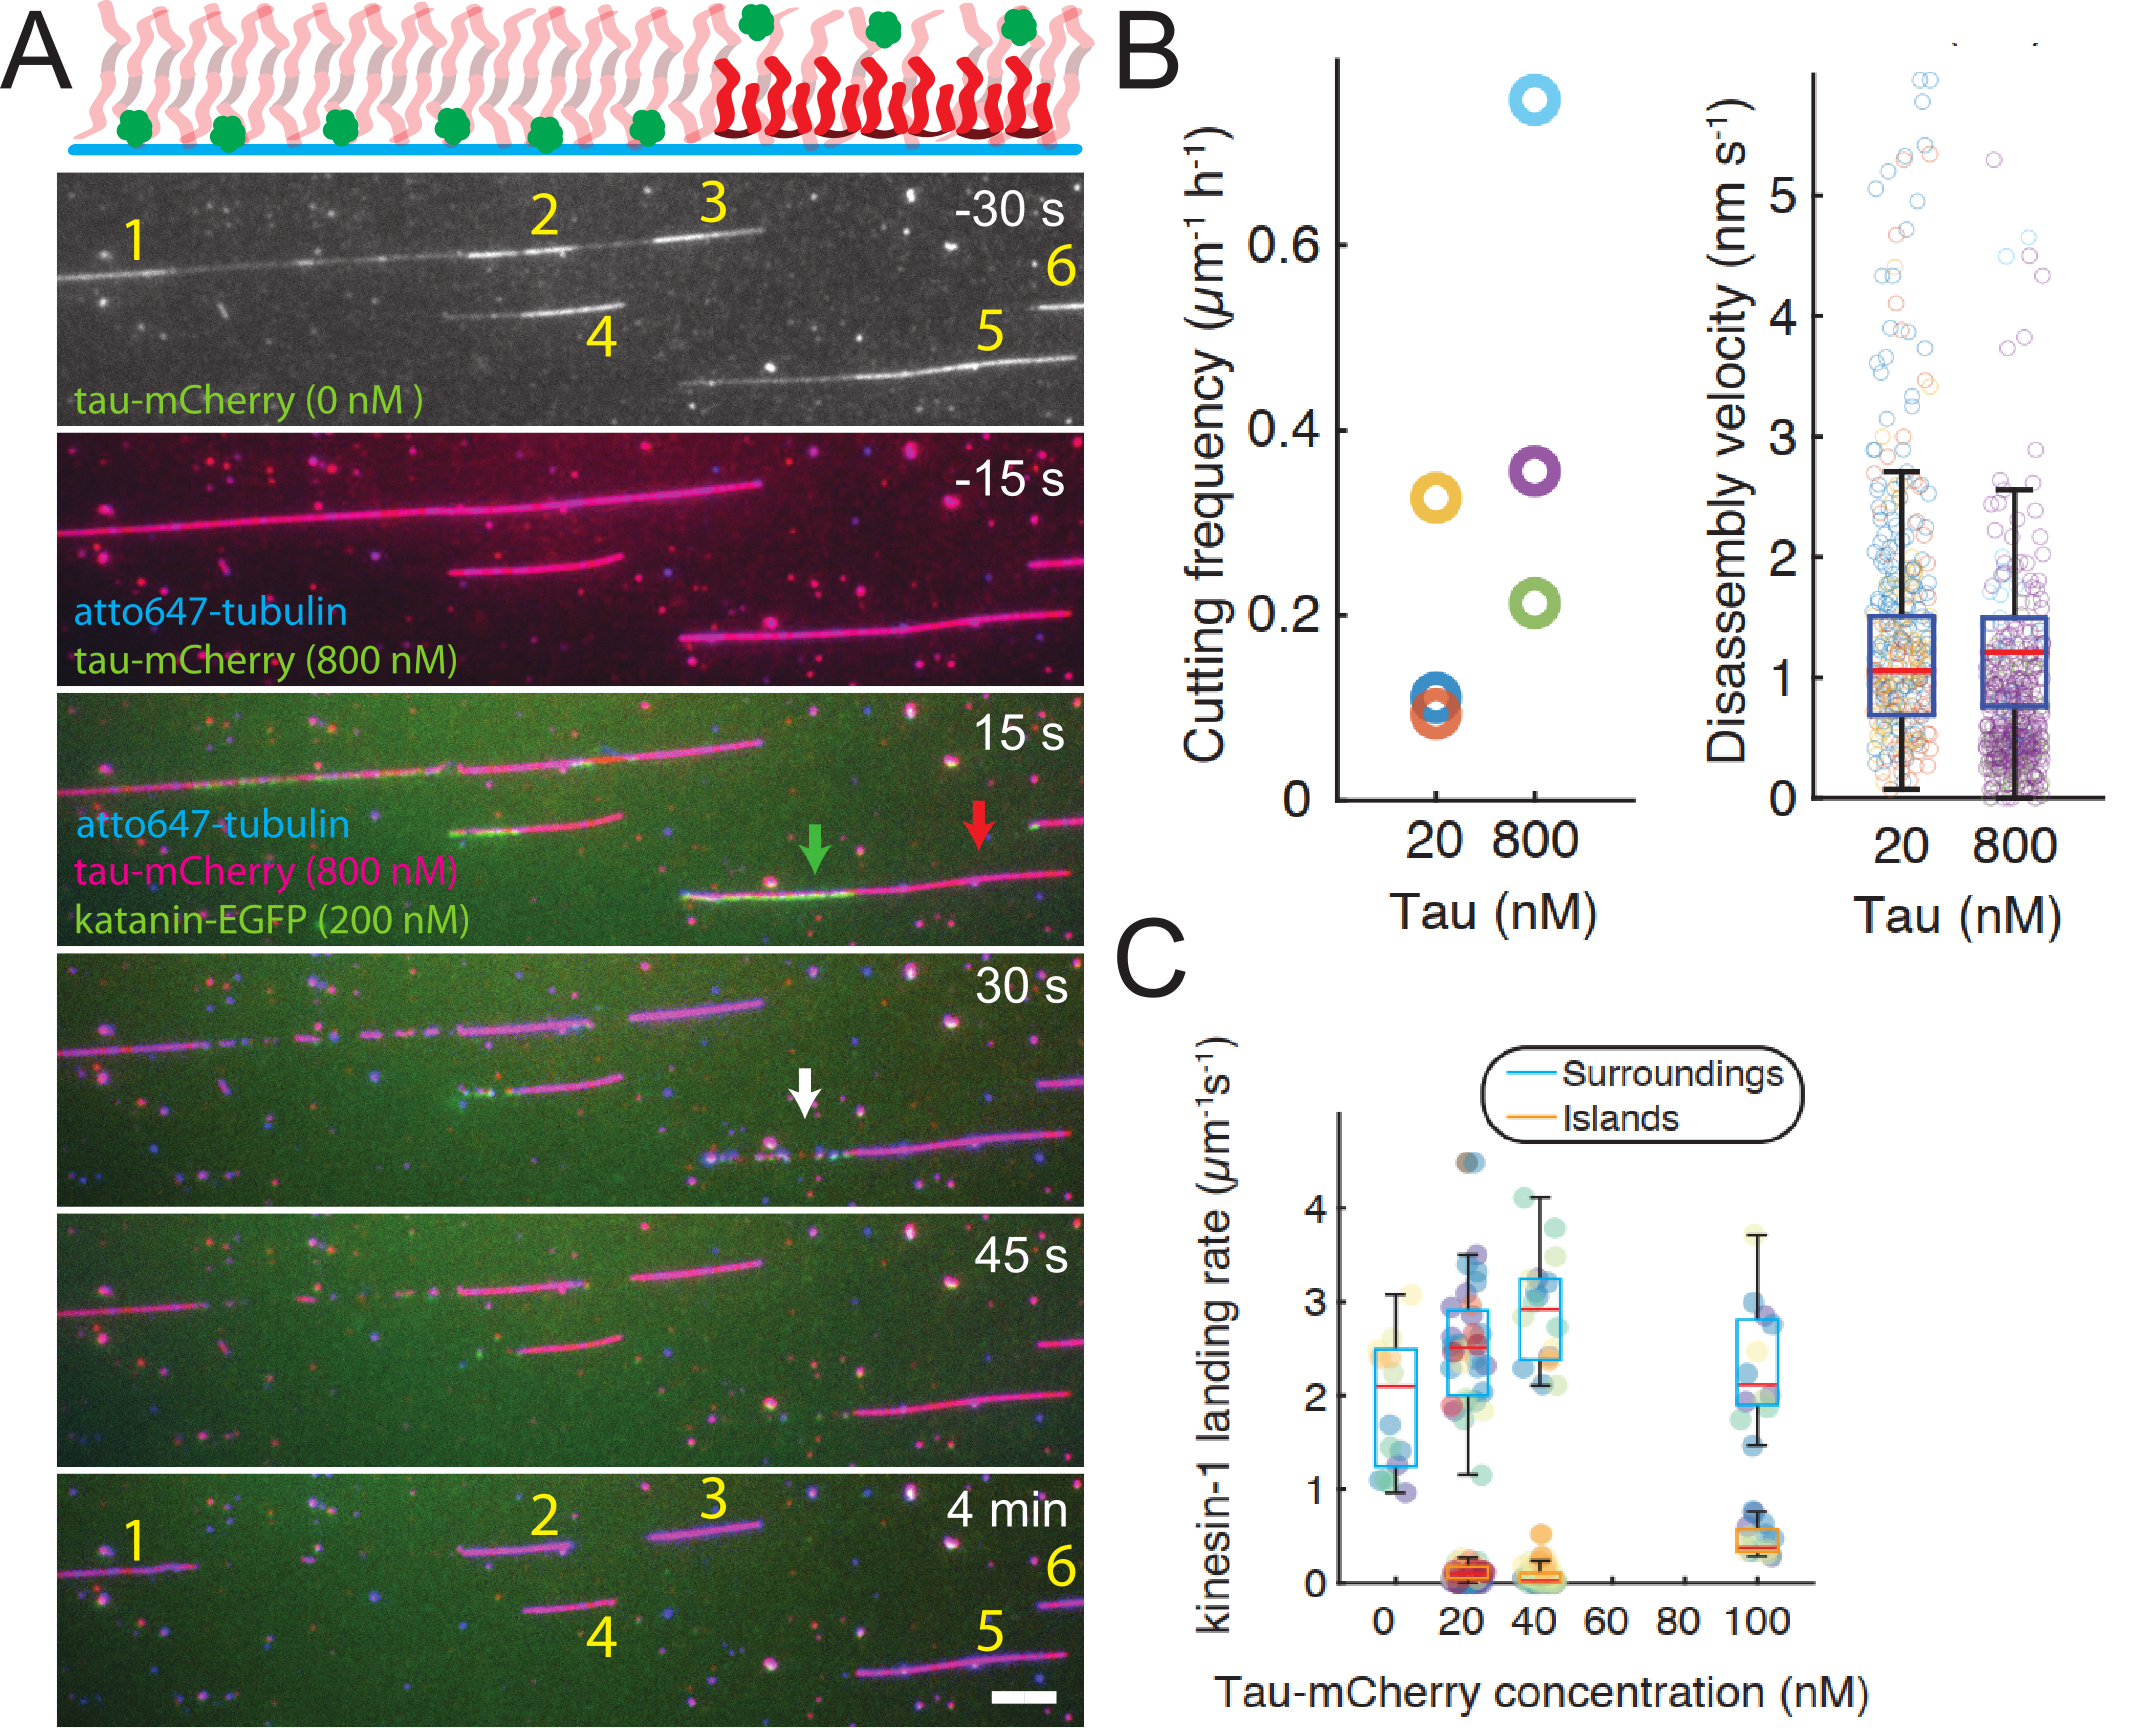
\includegraphics[width=1\linewidth]{Figures/tau6.png}
\caption[Microtubule shielding depends on tau cohesion of the islands.]{ 
\textbf{Microtubule shielding depends on tau cohesion of the islands.} (A) Fluorescence micrographs showing katanin-GFP-driven (green) severing of Atto-647-microtubules (blue) decorated with tau-mCherry islands (red) formed at 0.8 µM tau-mCherry concentration. The island positions (indicated by numbers) were determined by a brief removal of tau-mCherry from solution (Methods). Katanin is recruited to regions outside of the islands (green arrow) and excluded form the islands (red arrow). Microtubule severing and disassembly occurred initially only in the regions outside of the islands (example indicated by white arrow). Compare to the Figure \ref{tau3}B. Scale bar 2 µm. (B) Boxplot of katanin-mediated disassembly velocities of stretches of microtubules covered by tau islands (evaluated per island boundary) and the rate of katanin-generated cuts occurring within them. Experiments had been conducted at two different concentrations of tau in solution. (C) Kinesin-1 landing rates inside and outside the islands formed at various tau-mCherry concentrations in solution (7 experiments at 0 nM, 10 experiments at 20 nM, 7 experiments at 40 nM, 6 experiments at 100nM).
	}\label{tau6}
\end{figure}
 Since the characteristic tau density of the islands is lower than that of the surrounding regions at physiological tau concentrations (Figure 5), we wondered if the discretely binding tau molecules in the island surroundings, at these concentrations, are sufficient for shielding the microtubule against microtubule severing. To test the shielding against katanin severing at physiological tau concentration we thus formed tau-mCherry islands at saturating conditions (0.8 µM). After 5 minutes of incubation we briefly removed tau-mCherry from solution to note the position of the islands, and then again re-introduced 0.8 µM tau-mCherry in the assay. We then exposed such tau-mCherry decorated microtubules to 0.2 µM katanin-GFP analogously to the experiment presented in Figure \ref{tau3}B. Strikingly, we observed qualitatively identical results as in the Figure \ref{tau3}B. Namely, regions surrounding the islands and occupied by the diffusible tau-mCherry phase were severed and rapidly disassembled, while microtubule regions shielded by the islands persisted (Figure \ref{tau6}). This shows that the density of tau on the microtubule surface is not the factor determining the shielding function of tau. Rather it is the cohesion between the tau molecules constituting the islands, which protects the microtubules. This conclusion is supported by our observation that increasing the tau concentration in solution did not substantially increase shielding against tau (Figure \ref{tau6}B) and kinesin-1 (Figure \ref{tau6}B). 

\subsection{Tau islands do not form at regions of high microtubule curvature}
\begin{figure}[h!]
\centering
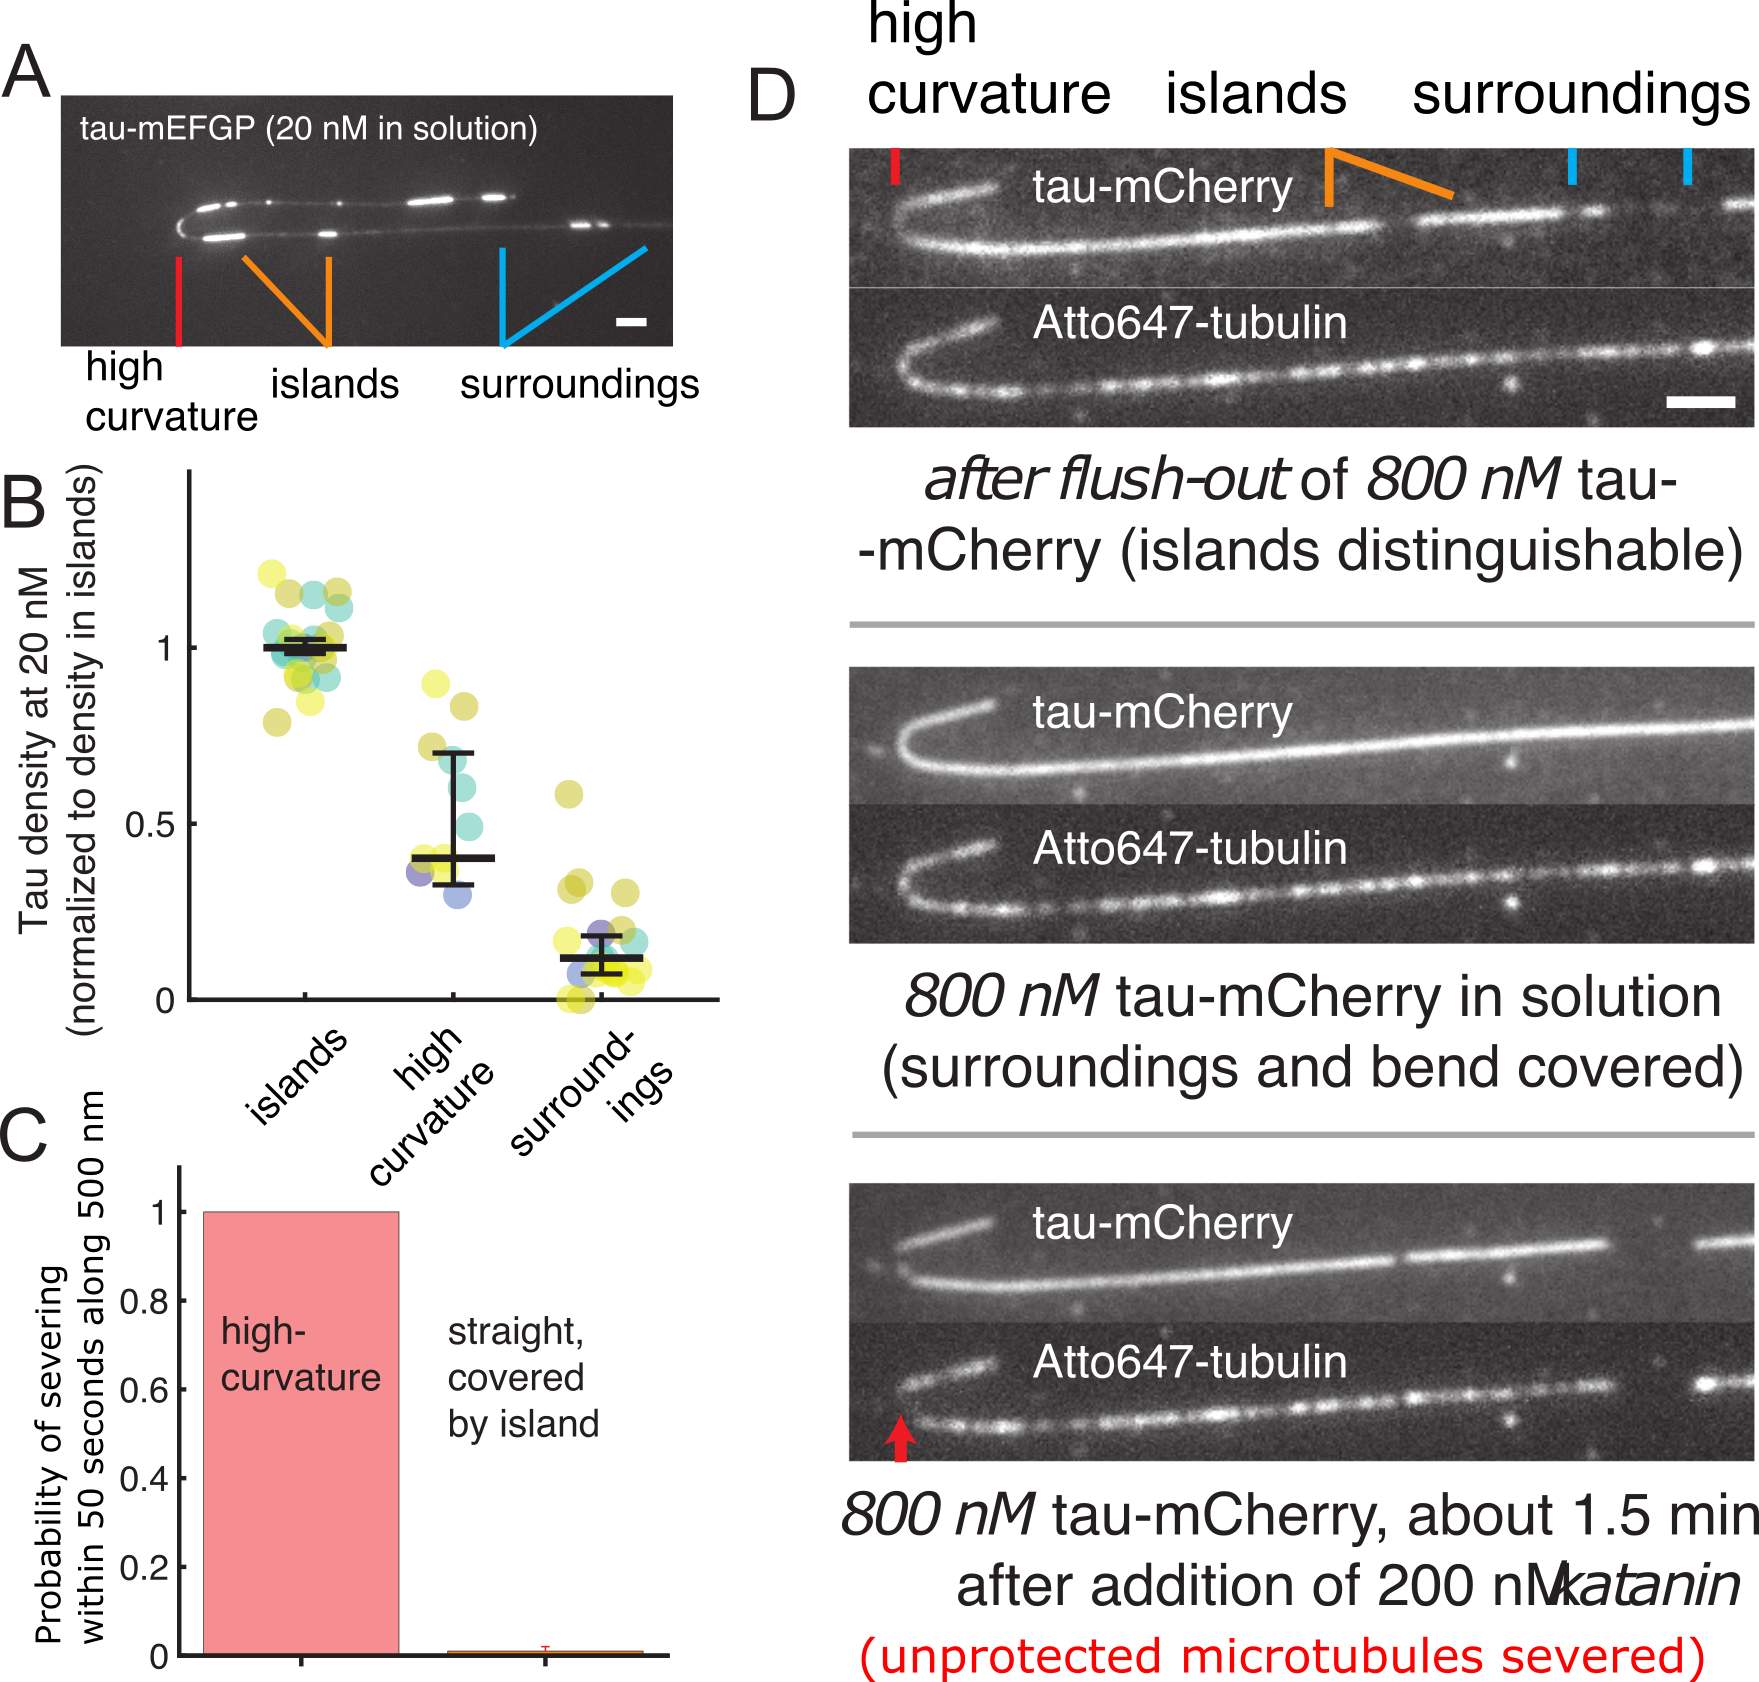
\includegraphics[scale=1]{Figures/tau7.png}
\caption[Tau islands do not form at regions of high microtubule curvature.]{
\textbf{Tau islands do not form at regions of high microtubule curvature.} (A) Fluorescence micrograph showing the tau-mEGFP signal on microtubules at 20 nM tau-mEGFP in solution. Tau islands have higher tau-mEGFP densities than the tau-mEGFP regions localizing to microtubule regions with high curvature. (B) Densities of tau-mEGFP outside the islands, inside the islands and in the regions of high curvature at 20 nM tau-mEGFP in solution (n = 11 high-curvature regions in 5 experiments). Points are color-coded by experiments, horizontal lines indicate the three quartiles, weighted such that each experiment has equal weight. (C) Probability of severing of highly curved microtubule regions and adjacent straight island-covered microtubule regions, within 150 s after the addition of katanin. The bars represent the probability averaged over n = 4 experiments (29 bends and 82 straight microtubules), error bars represent the S.D. Curved microtubule regions were always cut. (D) An experiment as analyzed in (C). Tau-mCherry islands on microtubules after the removal of 800 nM tau-mCherry from solution (upper panel); the same microtubule in presence of re-introduced 800 nM tau-mCherry in solution (middle panel); the same microtubule in presence of 200 nM katanin-GFP and 800 nM tau-mCherry. The red arrow highlights that the high curvature region  had been cut by katanin. This experiment had been repeated 4 times with similar results. Scale bars 2 µm.
	}\label{tau7}
\end{figure}
Earlier reports show that tau preferentially localized to highly-curved microtubules\parencite{Samsonov2004}. We indeed observed that regions of highly curved microtubules (radius < 2.5 µm) exhibited a tau density that was higher than in the surroundings, but lower than in the islands on straight microtubule regions (Figure \ref{tau7}A,B). The tau bound to highly curved microtubule regions also did not unbind as quickly as in the surroundings (Figure \ref{tau7}D, \ref{tau_s7}A,B). Importantly however, the highly curved regions were not protected from katanin-mediated severing (Figure \ref{tau7}C,D), demonstrating that tau molecules in the highly curved regions do not form a cohesive layer. Accordingly, in the curved regions tau-mEGFP binding was distinct from the island formation on straight microtubules, in that there was no growth at boundaries (Figure \ref{tau_s7}C). Combined, these experiments suggest that high curvatures of microtubules, though attracting tau, prevent the formation of cohesive tau islands.